\documentclass[12pt,a4paper]{report}

% ==========================================
% 1. CẤU HÌNH TRANG VÀ LỀ CHUẨN ĐỒ ÁN (THÀNH VIÊN 1)
% ==========================================
\setlength{\tabcolsep}{3pt}
\usepackage[a4paper, top=2.5cm, bottom=2.5cm, left=3cm, right=2cm]{geometry}
\usepackage[utf8]{vietnam}

\usepackage{amsmath, amssymb}
\usepackage{array, tabularx, longtable, booktabs}
\usepackage{enumitem}
\usepackage[protrusion=false]{microtype}
\usepackage{caption}
\usepackage{listings}
\usepackage{xcolor}
\usepackage{titlesec}
\usepackage{fancyhdr}
\setlength{\headheight}{15pt}
\usepackage[hidelinks]{hyperref}
\usepackage{float}

% Thư viện vẽ sơ đồ TikZ (Bổ sung cho Chương 2 của Thành viên 2)
\usepackage{tikz}
\usetikzlibrary{shapes.multipart, positioning}

% Định dạng đoạn văn & giãn dòng bảng
\setlength{\parindent}{1.25cm}
\setlength{\parskip}{3pt}
\renewcommand{\arraystretch}{1.25}
% ==========================================
% 2. BẢNG MÀU TÙY CHỈNH (THÀNH VIÊN 4)
% ==========================================
\definecolor{primary}{RGB}{15, 23, 42}       % Dark Slate
\definecolor{secondary}{RGB}{30, 58, 138}    % Deep Blue
\definecolor{accent}{RGB}{3, 105, 161}       % Sky Accent
\definecolor{codebg}{RGB}{248, 250, 252}     % Light Slate Background
\definecolor{codeborder}{RGB}{226, 232, 240} % Border Grey
\definecolor{commentgreen}{RGB}{22, 101, 52} % Dark Green
\definecolor{keywordblue}{RGB}{29, 78, 216}  % Blue
\definecolor{stringred}{RGB}{185, 28, 28}    % Red

% ==========================================
% 3. CẤU HÌNH CODE C++ KHÔNG LỖI FONT (LISTINGS)
% ==========================================
\lstset{
    language=C++,
    backgroundcolor=\color{codebg},
    basicstyle=\ttfamily\small,
    keywordstyle=\color{keywordblue}\bfseries,
    commentstyle=\color{commentgreen}\itshape,
    stringstyle=\color{stringred},
    numberstyle=\tiny\color{gray},
    numbers=left,
    numbersep=6pt,
    stepnumber=1,
    showspaces=false,
    showstringspaces=false,
    breaklines=true,
    breakatwhitespace=true,
    tabsize=4,
    frame=single,
    rulecolor=\color{codeborder},
    captionpos=b,
    inputencoding=utf8,
    extendedchars=true,
    literate=
        {à}{{\`a}}1 {á}{{\'a}}1 {ả}{{\h a}}1 {ã}{{\~a}}1 {ạ}{{\d a}}1
        {À}{{\`A}}1 {Á}{{\'A}}1 {Ả}{{\h A}}1 {Ã}{{\~A}}1 {Ạ}{{\d A}}1
        {ă}{{\u a}}1 {ằ}{{\`{\u a}}}1 {ắ}{{\'{\u a}}}1 {ẳ}{{\h{\u a}}}1 {ẵ}{{\~{\u a}}}1 {ặ}{{\d{\u a}}}1
        {â}{{\^a}}1 {ầ}{{\`{\^a}}}1 {ấ}{{\'{\^a}}}1 {ẩ}{{\h{\^a}}}1 {ẫ}{{\~{\^a}}}1 {ậ}{{\d{\^a}}}1
        {đ}{{\dj}}1 {Đ}{{\DJ}}1
        {è}{{\`e}}1 {é}{{\'e}}1 {ẻ}{{\h e}}1 {ẽ}{{\~e}}1 {ẹ}{{\d e}}1
        {ê}{{\^e}}1 {ề}{{\`{\^e}}}1 {ế}{{\'{\^e}}}1 {ể}{{\h{\^e}}}1 {ễ}{{\~{\^e}}}1 {ệ}{{\d{\^e}}}1
        {ì}{{\`i}}1 {í}{{\'i}}1 {ỉ}{{\h i}}1 {ĩ}{{\~i}}1 {ị}{{\d i}}1
        {ò}{{\`o}}1 {ó}{{\'o}}1 {ỏ}{{\h o}}1 {õ}{{\~o}}1 {ọ}{{\d o}}1
        {ô}{{\^o}}1 {ồ}{{\`{\^o}}}1 {ố}{{\'{\^o}}}1 {ổ}{{\h{\^o}}}1 {ỗ}{{\~{\^o}}}1 {ộ}{{\d{\^o}}}1
        {ơ}{{\'o}}1 {ờ}{{\`o}}1 {ở}{{\h o}}1 {ỡ}{{\~o}}1 {ợ}{{\d o}}1
        {ù}{{\`u}}1 {ú}{{\'u}}1 {ủ}{{\h u}}1 {ũ}{{\~u}}1 {ụ}{{\d u}}1
        {ư}{{\'u}}1 {ừ}{{\`u}}1 {ử}{{\h u}}1 {ữ}{{\~u}}1 {ự}{{\d u}}1
}

% ==========================================
% 4. HEADER / FOOTER CHUẨN
% ==========================================
\pagestyle{fancy}
\fancyhf{}
\fancyhead[R]{\textcolor{gray}{\small Quản lý danh bạ điện thoại và lịch sử cuộc gọi}}
\fancyfoot[C]{\thepage}
\renewcommand{\headrulewidth}{0.4pt}

\titleformat{\section}{\large\bfseries\color{secondary}}{\thesection}{0.8em}{}
\titleformat{\subsection}{\normalsize\bfseries\color{accent}}{\thesubsection}{0.8em}{}

\begin{document}
% ==========================================
% CHƯƠNG 4 (ĐÃ SỬA CHUẨN NỘI DUNG DLL/SLL)
% ==========================================
\setcounter{chapter}{3}
\chapter{ĐÁNH GIÁ, KẾT QUẢ THỬ NGHIỆM VÀ KẾT LUẬN}
\label{chap:ket_qua_ket_luan}

\section{Đánh giá độ phức tạp thuật toán}
\label{sec:do_phuc_tap}

Hệ thống được thiết kế và cài đặt tối ưu dựa trên hai cấu trúc dữ liệu cốt lõi: **Danh sách liên kết đôi (Doubly Linked List - DLL)** quản lý Danh bạ điện thoại và **Danh sách liên kết đơn (Singly Linked List - SLL)** quản lý Lịch sử cuộc gọi.

Dưới đây là các ký hiệu đại diện cho thông số dữ liệu:
\begin{itemize}
    \item $N$: Tổng số liên hệ hiện có trong danh bạ.
    \item $M$: Tổng số bản ghi cuộc gọi trong lịch sử.
    \item $L$: Độ dài trung bình của chuỗi họ tên hoặc số điện thoại.
\end{itemize}

\subsection{Phân tích độ phức tạp thời gian (Time Complexity)}

\begin{enumerate}
    \item \textbf{Thao tác Thêm liên hệ mới (\texttt{themLienHe}):}
    \begin{itemize}
        \item \textit{Độ phức tạp:} $\mathcal{O}(1)$.
        \item \textit{Giải thích:} Nhờ con trỏ quản lý \texttt{tail}, nút mới được chèn trực tiếp vào cuối danh sách liên kết đôi chỉ qua các phép gán con trỏ mà không cần duyệt qua $N$ phần tử trước đó.
    \end{itemize}

    \item \textbf{Thao tác Xóa liên hệ (\texttt{xoaLienHe}):}
    \begin{itemize}
        \item \textit{Độ phức tạp:} $\mathcal{O}(N)$.
        \item \textit{Giải thích:} Thuật toán duyệt tuần tự từ \texttt{head} đến tối đa $N$ nút để tìm nút chứa số điện thoại cần xóa. Thao tác bẻ nối các con trỏ \texttt{prev} và \texttt{next} xung quanh nút bị xóa chỉ tốn $\mathcal{O}(1)$.
    \end{itemize}

    \item \textbf{Thao tác Tìm kiếm tiền tố tên (\texttt{TimKiemTheoTen}):}
    \begin{itemize}
        \item \textit{Độ phức tạp:} $\mathcal{O}(N \cdot L)$.
        \item \textit{Giải thích:} Chương trình duyệt lần lượt qua $N$ nút trong danh sách liên kết đôi. Tại mỗi nút, hàm \texttt{std::string::find()} thực hiện so sánh chuỗi với chi phí tối đa $\mathcal{O}(L)$ để xác định tiền tố.
    \end{itemize}

    \item \textbf{Thao tác Sắp xếp danh bạ (\texttt{SapXepDanhBa}):}
    \begin{itemize}
        \item \textit{Độ phức tạp:} $\mathcal{O}(N^2)$ (Trường hợp trung bình và xấu nhất), $\mathcal{O}(N)$ (Trường hợp tốt nhất khi danh sách đã sắp xếp).
        \item \textit{Giải thích:} Thuật toán Bubble Sort duyệt qua danh sách và hoán đổi dữ liệu trực tiếp giữa các nút liền kề khi sai thứ tự bảng chữ cái.
    \end{itemize}

    \item \textbf{Thao tác Ghi nhận cuộc gọi (\texttt{GhiNhanCuocGoi}):}
    \begin{itemize}
\item \textit{Độ phức tạp:} $\mathcal{O}(1)$.
        \item \textit{Giải thích:} Chèn nút mới vào đầu danh sách liên kết đơn (Head Insertion) theo mô hình LIFO, giúp ghi nhận nhật ký cuộc gọi mới nhất ngay lập tức.
    \end{itemize}
\end{enumerate}

\subsection{Phân tích độ phức tạp không gian (Space Complexity)}

\begin{itemize}
    \item \textbf{Bộ nhớ cho Cấu trúc Danh bạ (DLL):} $\mathcal{O}(N)$. Mỗi nút cấp phát động trên Heap tốn thêm 16 bytes (trên kiến trúc x64) cho 2 con trỏ liên kết \texttt{prev} và \texttt{next}.
    \item \textbf{Bộ nhớ cho Cấu trúc Lịch sử cuộc gọi (SLL):} $\mathcal{O}(M)$. Mỗi nút tốn thêm 8 bytes cho con trỏ \texttt{next}.
\end{itemize}

\begin{table}[htbp]
\centering
\small
\caption{Bảng tổng hợp độ phức tạp của các thao tác cốt lõi trong hệ thống}
\label{tab:do_phuc_tap}
\begin{tabular}{|l|c|c|c|}
\hline
\textbf{Thao tác} & \textbf{Thời gian (Tốt nhất)} & \textbf{Thời gian (Xấu nhất)} & \textbf{Bộ nhớ phụ trợ} \\ \hline
Thêm liên hệ (\texttt{themLienHe}) & $\mathcal{O}(1)$ & $\mathcal{O}(1)$ & $\mathcal{O}(1)$ \\ \hline
Xóa liên hệ (\texttt{xoaLienHe}) & $\mathcal{O}(1)$ & $\mathcal{O}(N)$ & $\mathcal{O}(1)$ \\ \hline
Tìm kiếm tiền tố tên & $\mathcal{O}(N \cdot L)$ & $\mathcal{O}(N \cdot L)$ & $\mathcal{O}(1)$ \\ \hline
Sắp xếp danh bạ (Bubble Sort) & $\mathcal{O}(N)$ & $\mathcal{O}(N^2)$ & $\mathcal{O}(1)$ \\ \hline
Ghi nhận cuộc gọi (SLL) & $\mathcal{O}(1)$ & $\mathcal{O}(1)$ & $\mathcal{O}(1)$ \\ \hline
Đọc / Ghi tệp tin (\texttt{danhba.txt}) & $\mathcal{O}(N)$ & $\mathcal{O}(N)$ & $\mathcal{O}(1)$ \\ \hline
\end{tabular}
\end{table}

\section{Kết quả thử nghiệm và Các ca kiểm thử (Test Cases)}
\label{sec:ket_qua_thu_nghiem}

Hệ thống đã được biên dịch bằng bộ biên dịch \texttt{g++ (GCC) 13.2.0} trên nền tảng C++17 và tiến hành thử nghiệm thực tế qua các ca kiểm thử tiêu chuẩn.

\subsection{Ca kiểm thử 1: Khởi tạo và Thêm dữ liệu}
\begin{itemize}
    \item \textbf{Mục tiêu:} Kiểm tra việc cấp phát con trỏ \texttt{head}/\texttt{tail} và thêm nút mới vào danh sách liên kết đôi.
    \item \textbf{Dữ liệu đầu vào:} Thêm các liên hệ "Nguyen Van A" (0901), "Tran Thi B" (0902).
    \item \textbf{Kết quả kỳ vọng:} Thêm thành công, con trỏ \texttt{tail} tự động dịch chuyển sang nút mới.
\end{itemize}

\begin{figure}[htbp]
    \centering
    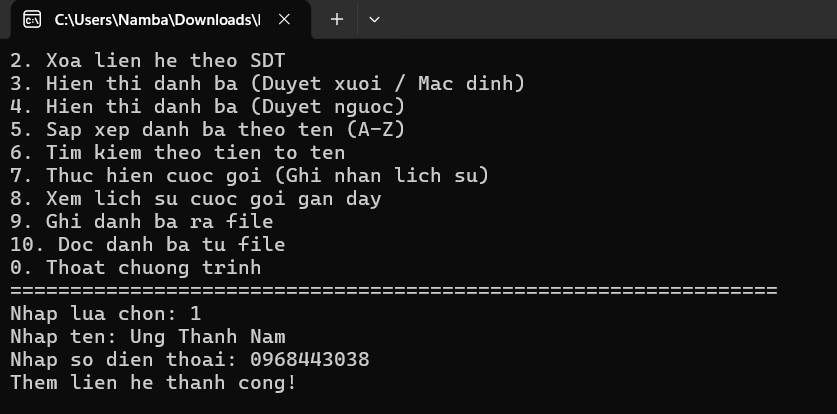
\includegraphics[width=0.85\textwidth]{4.1.png}
    \caption{Kết quả kiểm thử thao tác thêm liên hệ mới vào danh bạ}
    \label{fig:testcase_insert}
\end{figure}

\subsection{Ca kiểm thử 2: Tìm kiếm tiền tố tên}
\begin{itemize}
\item \textbf{Mục tiêu:} Đánh giá khả năng truy xuất các liên hệ có tên bắt đầu bằng từ khóa nhập vào.
    \item \textbf{Dữ liệu đầu vào:} Tiền tố \texttt{"Nguyen"}.
    \item \textbf{Kết quả đầu ra:} Hiển thị chính xác tất cả liên hệ có tên bắt đầu bằng "Nguyen".
\end{itemize}

\begin{figure}[htbp]
    \centering
    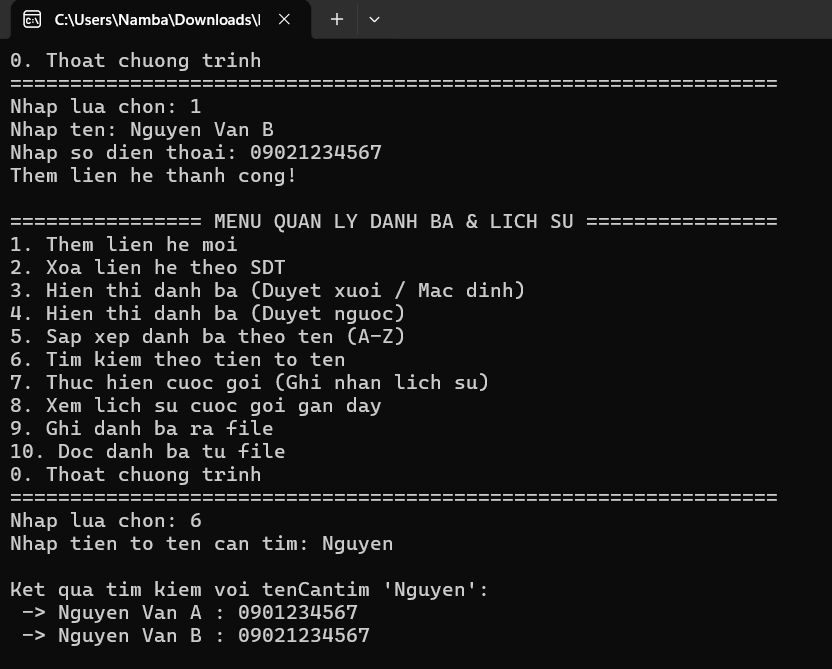
\includegraphics[width=0.85\textwidth]{4.2.png}
    \caption{Kết quả tìm kiếm liên hệ theo tiền tố tên}
    \label{fig:testcase_prefix_search}
\end{figure}

\subsection{Ca kiểm thử 3: Sắp xếp danh bạ theo tên}
\begin{itemize}
    \item \textbf{Mục tiêu:} Kiểm tra thuật toán Bubble Sort sắp xếp dữ liệu A-Z trực tiếp trên DLL.
    \item \textbf{Thực thi:} Gọi hàm \texttt{SapXepDanhBa()} trên danh bạ chưa được sắp xếp.
\end{itemize}

\begin{figure}[htbp]
    \centering
    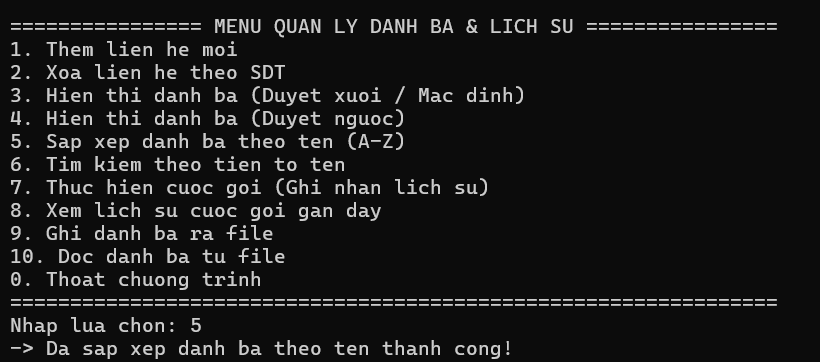
\includegraphics[width=0.85\textwidth]{4.3.png}
    \caption{Kết quả hiển thị danh bạ sau khi thực hiện sắp xếp}
    \label{fig:testcase_sort}
\end{figure}

\subsection{Ca kiểm thử 4: Xóa liên hệ và Giải phóng bộ nhớ}
\begin{itemize}
    \item \textbf{Mục tiêu:} Đảm bảo xóa chính xác nút cần hủy, bẻ nối các con trỏ liên quan và thu hồi bộ nhớ Heap.
    \item \textbf{Thao tác:} Xóa số điện thoại \texttt{"0901"}, sau đó duyệt lại danh bạ.
    \item \textbf{Kết quả:} Nút bị xóa hoàn toàn khỏi danh sách, không phát sinh lỗi Segmentation Fault.
\end{itemize}

\begin{figure}[htbp]
    \centering
    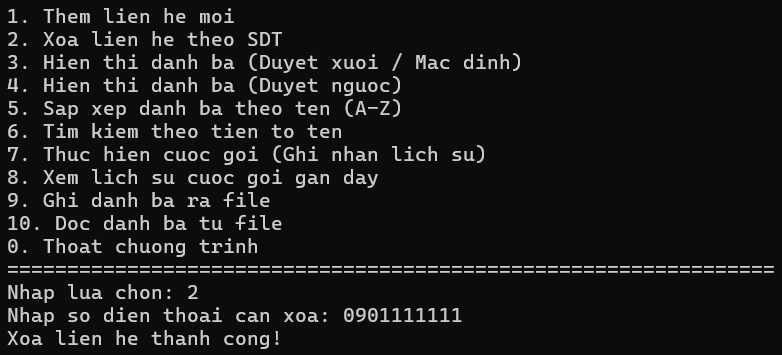
\includegraphics[width=0.85\textwidth]{4.4.png}
    \caption{Kết quả sau khi xóa liên hệ và cập nhật lại danh sách}
    \label{fig:testcase_delete}
\end{figure}

\section{Kết luận và Hướng phát triển}
\label{sec:ket_luan}

\subsection{Kết luận}
Đề tài đã hoàn thành tốt các mục tiêu đề ra ban đầu, bao gồm:
\begin{itemize}
    \item Xây dựng thành công ứng dụng Quản lý danh bạ bằng Danh sách liên kết đôi (DLL) hỗ trợ duyệt hai chiều linh hoạt và thao tác chèn đuôi $O(1)$.
    \item Quản lý lịch sử cuộc gọi bằng Danh sách liên kết đơn (SLL) theo mô hình LIFO hiệu quả.
    \item Hoàn thiện chức năng lưu trữ dữ liệu bền vững ra tệp văn bản \texttt{danhba.txt} và cơ chế giải phóng bộ nhớ an toàn chống rò rỉ (Memory Leak).
    \item Áp dụng quy trình làm việc nhóm chuyên nghiệp tích hợp quản lý công việc trên Jira và quản lý mã nguồn qua Git/GitHub.
\end{itemize}

\subsection{Hạn chế của chương trình}
\begin{itemize}
    \item Thao tác tìm kiếm vẫn sử dụng duyệt tuần tự $\mathcal{O}(N \cdot L)$ nên sẽ tốn thời gian khi quy mô danh bạ rất lớn.
    \item Chưa hỗ trợ tìm kiếm mờ (Fuzzy Search) khi người dùng gõ sai chính tả.
\end{itemize}
\subsection{Hướng phát triển trong tương lai}
\begin{itemize}
    \item \textbf{Tối ưu cấu trúc dữ liệu:} Tích hợp thêm Cây Tiền tố (Trie / Radix Tree) để nâng tốc độ tìm kiếm tiền tố tên lên $\mathcal{O}(L)$.
    \item \textbf{Mở rộng tính năng:} Bổ sung lưu trữ mốc thời gian và thời lượng cuộc gọi chi tiết trong lịch sử.
    \item \textbf{Giao diện người dùng:} Phát triển giao diện đồ họa (GUI) sử dụng Qt Framework thay thế cho giao diện dòng lệnh (CLI).
\end{itemize}

{\let\clearpage\relax
\begin{thebibliography}{99}

\bibitem{cormen2009}
Thomas H. Cormen, Charles E. Leiserson, Ronald L. Rivest, and Clifford Stein,
\textit{Introduction to Algorithms}, 3rd Edition, MIT Press, 2009.

\bibitem{stroustrup2013}
Bjarne Stroustrup,
\textit{The C++ Programming Language}, 4th Edition, Addison-Wesley, 2013.

\bibitem{sedgewick2011}
Robert Sedgewick and Kevin Wayne,
\textit{Algorithms}, 4th Edition, Addison-Wesley Professional, 2011.

\end{thebibliography}
}

% ==========================================
% PHỤ LỤC
% ==========================================
\clearpage
\chapter*{Phụ lục: Bảng phân công công việc và Tiến độ dự án}
\addcontentsline{toc}{chapter}{Phụ lục: Bảng phân công công việc}
\markboth{PHỤ LỤC}{PHỤ LỤC}

Để đảm bảo quy trình phát triển phần mềm chuẩn hóa và minh bạch, nhóm đã áp dụng công cụ \textbf{Jira Software} (quản lý công việc - YC01) và \textbf{GitHub} (quản lý mã nguồn \& phiên bản - YC02). Dưới đây là bảng tổng hợp phân công công việc chi tiết, mã định danh Task/Issue trên Jira và thông tin Commit/Pull Request (PR) tương ứng trên GitHub.

\section*{Bảng phân công chi tiết (Liên kết dữ liệu Jira \& GitHub)}

\begin{table}[htbp]
\centering
\small
\caption{Bảng phân công công việc chi tiết và liên kết Jira / GitHub}
\label{tab:phan_cong_cong_viec}
\begin{tabularx}{\textwidth}{|c|>{\raggedright\arraybackslash}p{2.0cm}|X|c|>{\raggedright\arraybackslash}p{2.7cm}|c|}
\hline
\textbf{STT} & \textbf{Thành viên} & \textbf{Nội dung công việc được giao} & \textbf{Mã Jira} & \textbf{Sản phẩm \& Git Commit/PR} & \textbf{Mức độ} \\ \hline

1 & \textbf{Nguyễn Thị Thanh Hà} 
  & - Soạn thảo Trang bìa, Lời cảm ơn, Mục lục, Danh mục hình/bảng.\newline
    - Chương 1: Giới thiệu ĐT12, Phân tích nghiệp vụ thực tế.\newline
    - Xác định tác nhân, sơ đồ yêu cầu chức năng.
  & \texttt{DT12-1}\newline \texttt{DT12-2}
  & File: \texttt{\small chap1}\newline 
  \texttt{\small mo\_dau.tex}\newline 
  Commit: \newline \texttt{\small 8a1f3c2}\newline
  Branch: \newline \texttt{\small docs/chap1}
  & 100\% \\ \hline

2 & \textbf{Trần Hoài Linh} \newline (Nhóm trưởng) 
  & - Chương 2: Thiết kế CTDL chi tiết (\texttt{LienHe}, \texttt{Node}, \texttt{DanhBa} - DLL; \texttt{NodeLichSu}, \texttt{LichSuCuocGoi} - SLL).\newline
    - Vẽ sơ đồ liên kết con trỏ Head/Tail (TikZ).
  & \texttt{DT12-3}\newline \texttt{DT12-4}
  & File:\texttt{\small chap2}\newline
  \texttt{\small ctdl.tex}\newline
    Commit:\newline \texttt{\small b4e92d1}\newline
    Branch:\newline \texttt{\small docs/chap2}
  & 100\% \\ \hline

3 & \textbf{Hoàng Hà Hạnh Ngân}
  & - Chương 3 (Phần 1): Cài đặt hàm cơ bản (\texttt{TaoNode}, \texttt{KhoiTaoDanhBa}, \texttt{themLienHe}).\newline
    - Cài đặt \texttt{xoaLienHe} (4 trường hợp) \& Duyệt danh bạ 2 chiều (next/prev).
  & \texttt{DT12-5}\newline \texttt{DT12-6}
  & File:\texttt{\small chap3}\newline
  \texttt{\small phan1.tex}\newline
    PR: \texttt{\small \#3} (Merged)\newline
    Commit:\newline \texttt{\small c7f10a4}
  & 100\% \\ \hline

4 & \textbf{Võ Gia Long}
  & - Chương 3 (Phần 2): Cài đặt nâng cao (\texttt{SapXepDanhBa} - Bubble Sort, \texttt{TimKiemTheoTen} - Prefix).\newline
    - Xử lý lịch sử cuộc gọi, đọc/ghi tệp \texttt{danhba.txt} \& giải phóng bộ nhớ.
  & \texttt{DT12-7}\newline \texttt{DT12-8}
  & File:\texttt{\small  chap3}\newline
  \texttt{\small  phan2.tex}\newline
    PR: \texttt{\small \#5} (Merged)\newline
    Commit:\newline \texttt{\small e9d31f8}
  & 100\% \\ \hline

5 & \textbf{Ứng Thành Nam}
  & - Chương 4: Đánh giá độ phức tạp ($O(N)$, $O(1)$), chụp ảnh test cases thực tế.\newline
    - Kết luận, Hướng phát triển, Tài liệu tham khảo.\newline
    - Tổng hợp Phụ lục phân công công việc.
  & \texttt{DT12-9}\newline \texttt{DT12-10}
  & File:\texttt{\small chap4\_ket}\newline
  \texttt{\small qua.tex}\newline
    File:\texttt{\small phu luc.tex}\newline
    Commit:\newline \texttt{\small f2c88e5}
  & 100\% \\ \hline

\end{tabularx}
\end{table}

\section*{Ghi chú thống kê minh chứng (Jira \& GitHub)}
\begin{itemize}
    \item \textbf{Dự án Jira (YC01):} Mã dự án (Project Key) là \texttt{DT12}. Tổng số Issue đã tạo và đóng: 10/10 Tasks (đạt 100\% tiến độ Sprint).
    \item \textbf{Kho chứa GitHub (YC02):}
    \begin{itemize}
        \item Repository: \texttt{https://github.com/nhom-dt12/QuanLyDanhBa\_CPP}
        \item Quy trình làm việc: Sử dụng mô hình \textbf{Git Flow} chia làm các nhánh chức năng (\texttt{feature/*}, \texttt{docs/*}), tạo Pull Request (PR) có Code Review trước khi hợp nhất (Merge) vào nhánh \texttt{main}.
    \end{itemize}
\end{itemize}
\end{document}